\chapter{Cost Functions}
Per valutare l'efficacia e le performance di un modello di deep learning usiamo una \textbf{cost function}.

Si usa il termine \textbf{loss function} o \textbf{error function} quando ci si riferisce un singolo esempio del training set,
mentre \textbf{cost function} sull'intero training set (o mini-batch).

La \textbf{cost function} misura l'errore tra il valore predetto dal modello e il valore di verità. 
L'obiettivo è quello di minimizzare o massimizzare questa funzione in modo da ridurre l'errore.

La \textbf{cost function} può contenere anche un termine di regolarizzazione.

\section{Loss Functions}
Sia $y = (y_1, y_2, ..., y_k)$ un vettore che rappresenta la distribuzione multinomiale di verità definito sulle etichette $1...k$.

Sia $\hat{y} = (\hat{y}_1, \hat{y}_2, ..., \hat{y}_k)$ il vettore delle predizioni, dove $\hat{y}_i = P(y = i | x, \theta)$.

\subsection*{Negative Log Likelihood}

$J(\theta) = -\mathbb{E}_{x, y \sim \hat{P}_{data}} \log(P_{model}(y | x))$

$J(\theta) = L_{neg\_likelihood}(y, \hat{y}) = - \sum_{i = 1}^k y_i \log (\hat{y}_i)$

\subsection*{Mean Squared Error (MSE)}

\begin{align*}
  L(y, \hat{y}) = \frac{1}{N} \sum_{i = 0}^N {(y - \hat{y}_i)^2}
\end{align*}

\subsection*{Mean Absolute Error (MAE)}

\begin{align*}
  L(y, \hat{y}) = \frac{1}{N} \sum_{i = 0}^N {|y - \hat{y}_i|}
\end{align*}

\section{Output Units}
La scelta della funzione di loss è legata all'unità di output.

\subsection{Linear - Distribuzione Gaussiana}
Spesso usato per ottenere la media di una distribuzione gaussiana condizionale.

$\hat{y} = w^T h + b$

\subsection{Sigmoid - Distribuzione Bernoulli}
Usata per predire il valore di una variabile binaria $\hat{y} \in [0, 1]$.

La distribuzione di output è una distribuzione di Bernoulli definita da $P(y = 1 | x)$.

La funzione sigmoide [\ref{eq:sigmoid}] ci permette di avere un gradiente forte quando abbiamo una predizione errata.

\begin{minipage}{0.6\linewidth}
  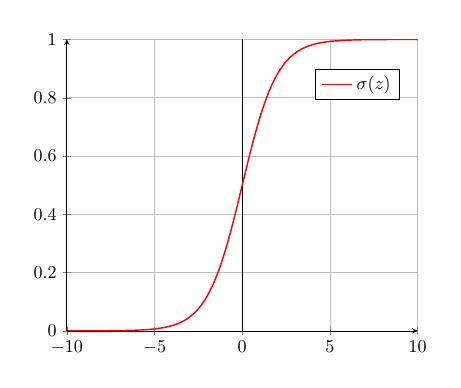
\begin{tikzpicture}[scale=0.65]
    \begin{axis}[
        axis x line = bottom,
        axis y line = left,
        grid = major,
        legend style={at={(0.95, 0.9)}},
      ]
      \addplot[thick, black, domain=-10:10, samples=2, forget plot] coordinates {(0,0)(0,1)};
      \addplot[thick, red, domain = -10:10, samples = 100]{1/(1+exp(-x))};
      \addlegendentry{$\sigma(z)$}
    \end{axis}
  \end{tikzpicture}
\end{minipage}
%
\begin{minipage}{0.3\linewidth}
  \begin{align}
    \sigma(z) = \frac{1}{1 + e^{-z}}
    \label{eq:sigmoid}
  \end{align}
\end{minipage}

Per prima cosa calcoliamo l'argomento $z = \omega^T h + b$ e poi applichiamo la sigmoide per trovare $\hat{y} = \sigma(\omega^T h + b)$.

$J(\theta) = -\mathbb{E}[\log P(y|x)]$
%
\begin{flalign*}
  &\log(\tilde{P}(y)) = yz \qquad \tilde{P}(y) = \exp(yz) &\\
  &P(y) = \frac{\exp(yz)}{\sum_{y'=0}^1 \exp(y'z)} = \frac{\exp(yz)}{1 + \exp(z)} = \sigma((2y - 1)z)&
\end{flalign*}
%
\begin{flalign*}
  &P(y=0) = \sigma((2 * 0 - 1) z) = \sigma(-z) &\\
  &P(y=1) = \sigma((2 * 1 - 1) z) = \sigma(z) &
\end{flalign*}
%
\begin{flalign*}
  J(\theta) = -\mathbb{E}[\log P(y|x)] = - \log \sigma((2 y - 1) z)
\end{flalign*}

\subsection{Softmax - Distribuzione Multinoulli}
Vogliamo rappresentare una distribuzione di probabilità $\hat{y}$ definita su una variabile discreta con n valori possibili.

$\hat{y} = P(y | x), \qquad \hat{y}_i = P(y = i | x),\; i = 1..n$

$z = w^T h + b \qquad z_i = \log(\tilde{P}(y = i | x))$

\begin{flalign*}
  &\text{Softmax}(z)_i = \frac{\exp(z_i)}{\sum_{j = 1}^n {\exp(z_j)}}&
\end{flalign*}

Calcolando il logaritmo della softmax possiamo riscriverla nel seguente modo:
\begin{flalign*}
  \log\text{Softmax}(z)_i &= \log(\exp(z_i)) - \log\sum_{j = 1}^n {\exp(z_j)}&\\
  &= z_i - \log\sum_{j = 1}^n {\exp(z_j)}&
\end{flalign*}
Quando massimizziamo, a valori alti del primo termine corrispondono valori bassi del secondo.
Quindi possiamo tenere in considerazione solo il $max_j z_j$.

Le altre funzioni di loss che non invertono l'esponenziale possono dare problemi di saturazione.
Quindi è stata definita una versione più stabile

$\text{Softmax}(z) = \text{Softmax}(z - max_i z_i)$

\subsection{Gaussian Mixtures}

